% Options for packages loaded elsewhere
\PassOptionsToPackage{unicode}{hyperref}
\PassOptionsToPackage{hyphens}{url}
%
\documentclass[
]{book}
\usepackage{amsmath,amssymb}
\usepackage{lmodern}
\usepackage{iftex}
\ifPDFTeX
  \usepackage[T1]{fontenc}
  \usepackage[utf8]{inputenc}
  \usepackage{textcomp} % provide euro and other symbols
\else % if luatex or xetex
  \usepackage{unicode-math}
  \defaultfontfeatures{Scale=MatchLowercase}
  \defaultfontfeatures[\rmfamily]{Ligatures=TeX,Scale=1}
\fi
% Use upquote if available, for straight quotes in verbatim environments
\IfFileExists{upquote.sty}{\usepackage{upquote}}{}
\IfFileExists{microtype.sty}{% use microtype if available
  \usepackage[]{microtype}
  \UseMicrotypeSet[protrusion]{basicmath} % disable protrusion for tt fonts
}{}
\makeatletter
\@ifundefined{KOMAClassName}{% if non-KOMA class
  \IfFileExists{parskip.sty}{%
    \usepackage{parskip}
  }{% else
    \setlength{\parindent}{0pt}
    \setlength{\parskip}{6pt plus 2pt minus 1pt}}
}{% if KOMA class
  \KOMAoptions{parskip=half}}
\makeatother
\usepackage{xcolor}
\usepackage{color}
\usepackage{fancyvrb}
\newcommand{\VerbBar}{|}
\newcommand{\VERB}{\Verb[commandchars=\\\{\}]}
\DefineVerbatimEnvironment{Highlighting}{Verbatim}{commandchars=\\\{\}}
% Add ',fontsize=\small' for more characters per line
\usepackage{framed}
\definecolor{shadecolor}{RGB}{248,248,248}
\newenvironment{Shaded}{\begin{snugshade}}{\end{snugshade}}
\newcommand{\AlertTok}[1]{\textcolor[rgb]{0.94,0.16,0.16}{#1}}
\newcommand{\AnnotationTok}[1]{\textcolor[rgb]{0.56,0.35,0.01}{\textbf{\textit{#1}}}}
\newcommand{\AttributeTok}[1]{\textcolor[rgb]{0.77,0.63,0.00}{#1}}
\newcommand{\BaseNTok}[1]{\textcolor[rgb]{0.00,0.00,0.81}{#1}}
\newcommand{\BuiltInTok}[1]{#1}
\newcommand{\CharTok}[1]{\textcolor[rgb]{0.31,0.60,0.02}{#1}}
\newcommand{\CommentTok}[1]{\textcolor[rgb]{0.56,0.35,0.01}{\textit{#1}}}
\newcommand{\CommentVarTok}[1]{\textcolor[rgb]{0.56,0.35,0.01}{\textbf{\textit{#1}}}}
\newcommand{\ConstantTok}[1]{\textcolor[rgb]{0.00,0.00,0.00}{#1}}
\newcommand{\ControlFlowTok}[1]{\textcolor[rgb]{0.13,0.29,0.53}{\textbf{#1}}}
\newcommand{\DataTypeTok}[1]{\textcolor[rgb]{0.13,0.29,0.53}{#1}}
\newcommand{\DecValTok}[1]{\textcolor[rgb]{0.00,0.00,0.81}{#1}}
\newcommand{\DocumentationTok}[1]{\textcolor[rgb]{0.56,0.35,0.01}{\textbf{\textit{#1}}}}
\newcommand{\ErrorTok}[1]{\textcolor[rgb]{0.64,0.00,0.00}{\textbf{#1}}}
\newcommand{\ExtensionTok}[1]{#1}
\newcommand{\FloatTok}[1]{\textcolor[rgb]{0.00,0.00,0.81}{#1}}
\newcommand{\FunctionTok}[1]{\textcolor[rgb]{0.00,0.00,0.00}{#1}}
\newcommand{\ImportTok}[1]{#1}
\newcommand{\InformationTok}[1]{\textcolor[rgb]{0.56,0.35,0.01}{\textbf{\textit{#1}}}}
\newcommand{\KeywordTok}[1]{\textcolor[rgb]{0.13,0.29,0.53}{\textbf{#1}}}
\newcommand{\NormalTok}[1]{#1}
\newcommand{\OperatorTok}[1]{\textcolor[rgb]{0.81,0.36,0.00}{\textbf{#1}}}
\newcommand{\OtherTok}[1]{\textcolor[rgb]{0.56,0.35,0.01}{#1}}
\newcommand{\PreprocessorTok}[1]{\textcolor[rgb]{0.56,0.35,0.01}{\textit{#1}}}
\newcommand{\RegionMarkerTok}[1]{#1}
\newcommand{\SpecialCharTok}[1]{\textcolor[rgb]{0.00,0.00,0.00}{#1}}
\newcommand{\SpecialStringTok}[1]{\textcolor[rgb]{0.31,0.60,0.02}{#1}}
\newcommand{\StringTok}[1]{\textcolor[rgb]{0.31,0.60,0.02}{#1}}
\newcommand{\VariableTok}[1]{\textcolor[rgb]{0.00,0.00,0.00}{#1}}
\newcommand{\VerbatimStringTok}[1]{\textcolor[rgb]{0.31,0.60,0.02}{#1}}
\newcommand{\WarningTok}[1]{\textcolor[rgb]{0.56,0.35,0.01}{\textbf{\textit{#1}}}}
\usepackage{graphicx}
\makeatletter
\def\maxwidth{\ifdim\Gin@nat@width>\linewidth\linewidth\else\Gin@nat@width\fi}
\def\maxheight{\ifdim\Gin@nat@height>\textheight\textheight\else\Gin@nat@height\fi}
\makeatother
% Scale images if necessary, so that they will not overflow the page
% margins by default, and it is still possible to overwrite the defaults
% using explicit options in \includegraphics[width, height, ...]{}
\setkeys{Gin}{width=\maxwidth,height=\maxheight,keepaspectratio}
% Set default figure placement to htbp
\makeatletter
\def\fps@figure{htbp}
\makeatother
\setlength{\emergencystretch}{3em} % prevent overfull lines
\providecommand{\tightlist}{%
  \setlength{\itemsep}{0pt}\setlength{\parskip}{0pt}}
\setcounter{secnumdepth}{-\maxdimen} % remove section numbering
\ifLuaTeX
  \usepackage{selnolig}  % disable illegal ligatures
\fi
\IfFileExists{bookmark.sty}{\usepackage{bookmark}}{\usepackage{hyperref}}
\IfFileExists{xurl.sty}{\usepackage{xurl}}{} % add URL line breaks if available
\urlstyle{same} % disable monospaced font for URLs
\hypersetup{
  hidelinks,
  pdfcreator={LaTeX via pandoc}}

\author{}
\date{\vspace{-2.5em}}

\begin{document}
\frontmatter

\mainmatter
\hypertarget{problema-3}{%
\chapter{Problema 3}\label{problema-3}}

Haga una modificación al problema de la empresa que se resuelve en el
codigo para resolución numérica del problema de inversión y reporte los
cambios que observe en las funciones valor y de política.

\hypertarget{paruxe1metros-econuxf3micos}{%
\subsection{Parámetros económicos}\label{paruxe1metros-econuxf3micos}}

Se modifican los parámetros económicos para ver el comportamiento de la
empresa con variaciones en sus costos.

\begin{Shaded}
\begin{Highlighting}[]
\CommentTok{\# Parámetros del modelo}
\NormalTok{Alpha }\OtherTok{\textless{}{-}} \FloatTok{0.5}  \CommentTok{\#Concavidad de la función producción}
\NormalTok{Costo\_Convexo }\OtherTok{\textless{}{-}} \DecValTok{2}  \CommentTok{\#Coeficiente de los costos de ajuste convexos}
\NormalTok{Beta }\OtherTok{\textless{}{-}} \FloatTok{0.95}
\NormalTok{Costo\_NoConvexo}\OtherTok{\textless{}{-}}\FloatTok{0.001}  \CommentTok{\#coeficiente de los costos de ajuste NO convexos}
\end{Highlighting}
\end{Shaded}

\begin{Shaded}
\begin{Highlighting}[]
\CommentTok{\# Parámetros del modelo modificado}
\NormalTok{Alphab }\OtherTok{\textless{}{-}} \FloatTok{0.5}  \CommentTok{\#Concavidad de la función producción}
\NormalTok{Costo\_Convexob }\OtherTok{\textless{}{-}} \DecValTok{20}  \CommentTok{\#Coeficiente de los costos de ajuste convexos}
\NormalTok{Betab }\OtherTok{\textless{}{-}} \FloatTok{0.95}
\NormalTok{Costo\_NoConvexob}\OtherTok{\textless{}{-}}\FloatTok{0.001}  \CommentTok{\#coeficiente de los costos de ajuste NO convexos}
\end{Highlighting}
\end{Shaded}

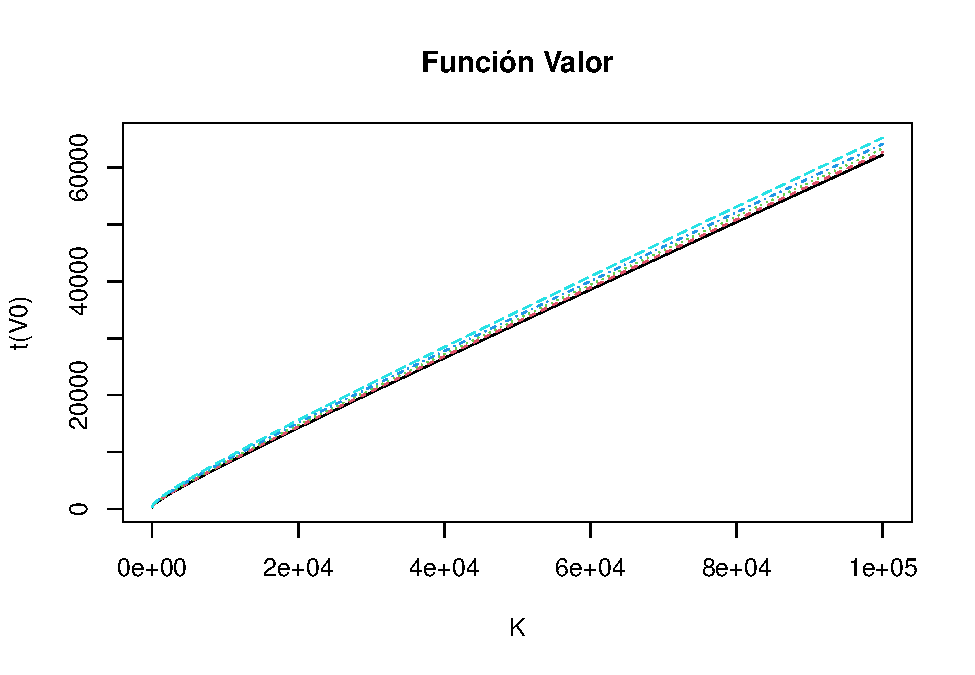
\includegraphics{Tarea-3-Ejercicio-3_files/figure-latex/unnamed-chunk-14-1.pdf}
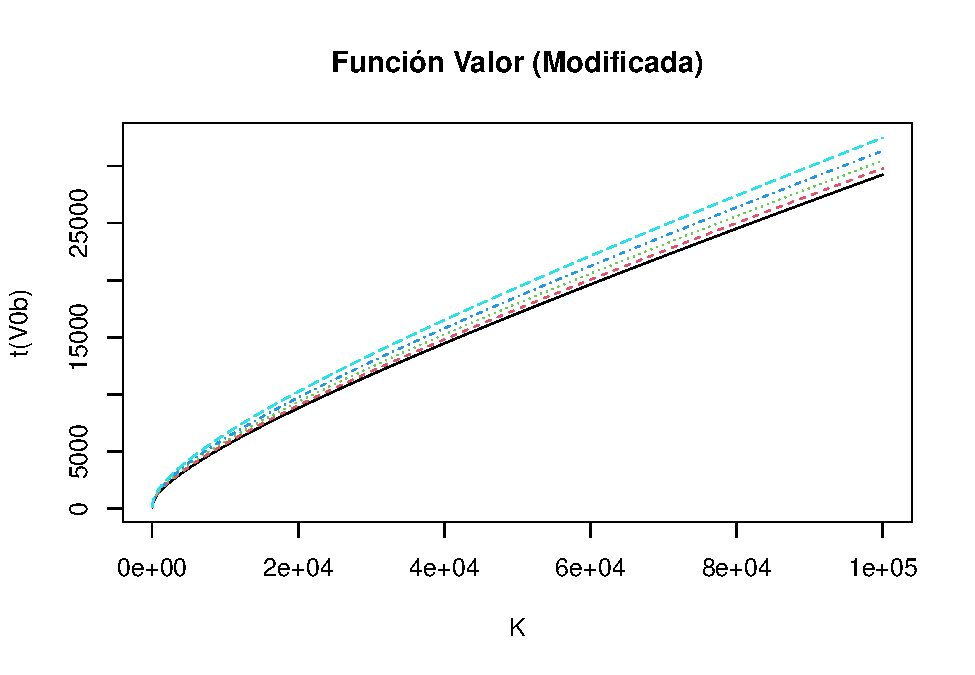
\includegraphics{Tarea-3-Ejercicio-3_files/figure-latex/unnamed-chunk-14-2.pdf}
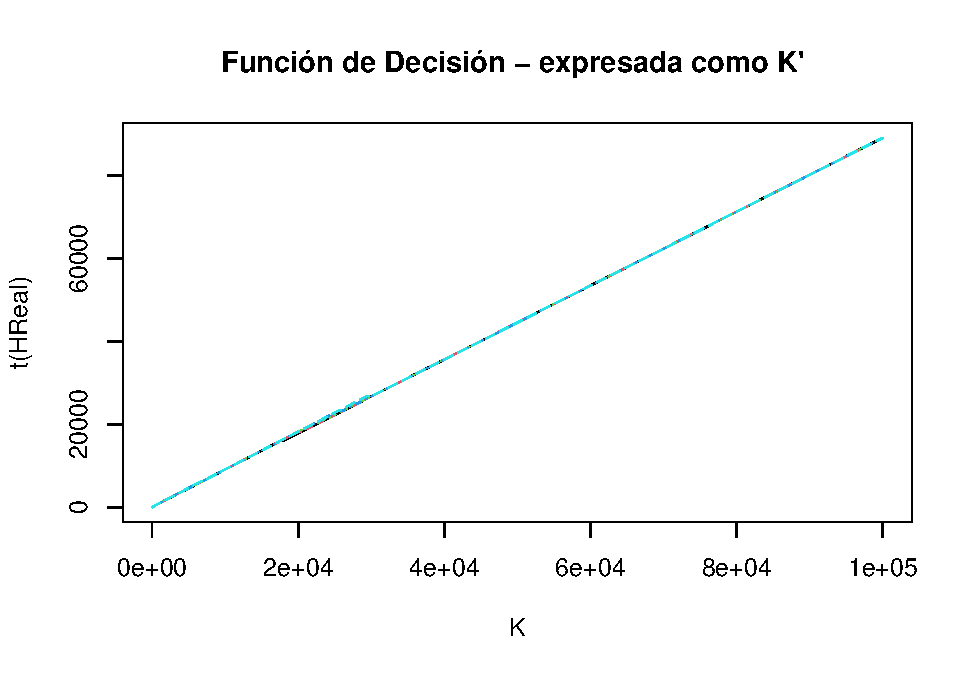
\includegraphics{Tarea-3-Ejercicio-3_files/figure-latex/unnamed-chunk-14-3.pdf}
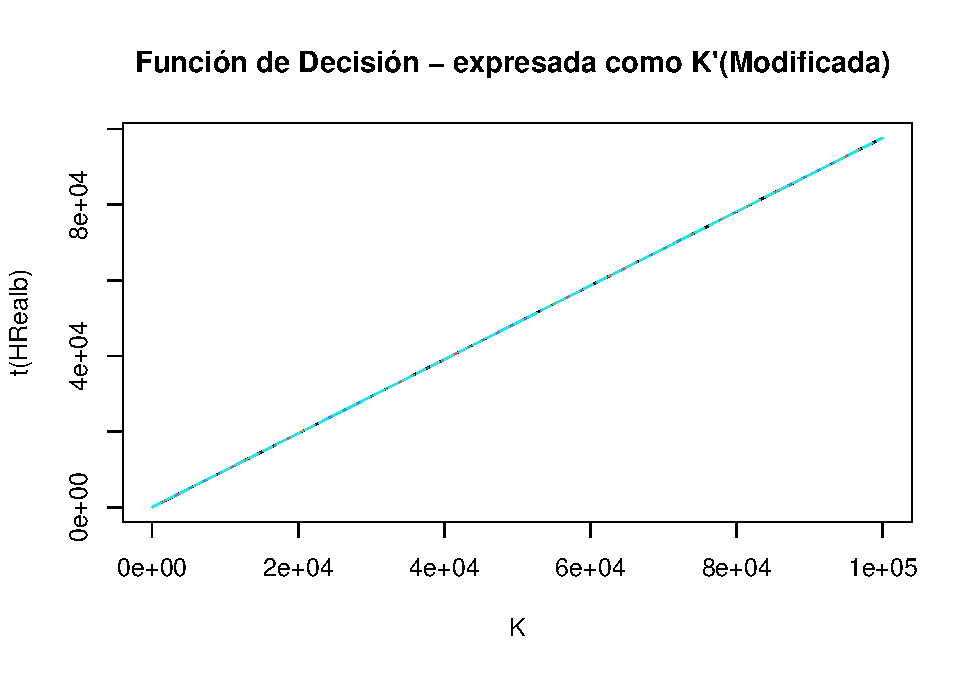
\includegraphics{Tarea-3-Ejercicio-3_files/figure-latex/unnamed-chunk-14-4.pdf}
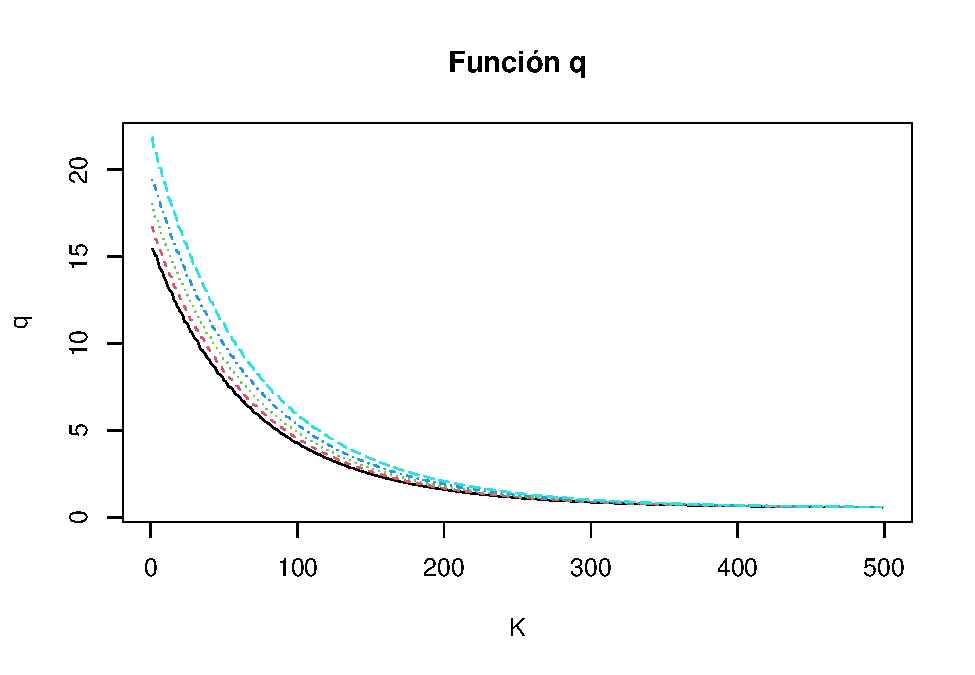
\includegraphics{Tarea-3-Ejercicio-3_files/figure-latex/unnamed-chunk-14-5.pdf}
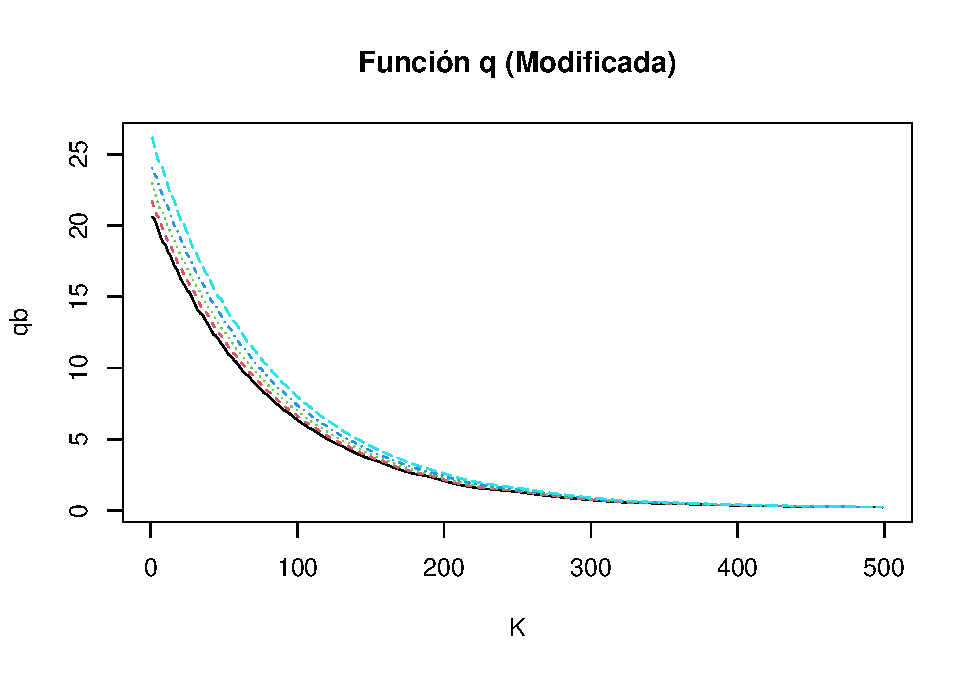
\includegraphics{Tarea-3-Ejercicio-3_files/figure-latex/unnamed-chunk-14-6.pdf}

Se aplica un aumento en el coeficiente de costos convexos de 2 a 20
unidades. Con estas modificacion podemos analizar el efecto que tienen
los costos en el estudio de la inversion. Aumentando el factor de costos
convexos 10 veces pasando de 2 a 20 unidades podemos notar una
disminucion de la funcion valor aproximadamente de la mitad del valor
inicial pasando de 60,000 a 30,000 unidades cuando el valor del capital
es de 100,000, mientras que la funcion de decision se mantiene sin
ninguna variacion.También podemos apreciar un aumento del valor ``q''
cuando aumentamos los costos convexos en aproximadamene 5 unidades
pasando de 15 a 20 en el caso de que el capital tiende a 0, lo que puede
interpretarse como : Un aumento de los costos convexos aumentan
relativamente el valor de ``q'' por lo que la empresa estará
sobrevalorada respecto al valor de su capital y sera menos atractivo de
invertir.

\backmatter
\end{document}
